% Proposed caption for the combined Figure 1 -- NOT yet inserted into the manuscript.
% Paper: "Safe Reinforcement Learning for Clinical Multi-Turn Agents Requires More Than Outcome Rewards"
% Figure: figs/figure1_combined.pdf
%
% Changes from the supplied draft (each forced by what the final graphic actually shows):
%   * B: added that the four rows are SINGLE REPRESENTATIVE ROLLOUTS (k=12 per condition), not modal or
%     aggregate behaviour -- the figure states this, so the caption must too.
%   * B: "oracle-grade sampled trajectory" qualified as oracle-grade BY REWARD with a different evidence
%     order, matching the on-figure annotation (it is not the oracle procedure).
%   * B: named the dx-13 case as held-out and rule-labelled, and named the reward values shown.
%   * C: described the dashed gold line (exact adaptive oracle on the same held-out cases, approx. 3.8
%     questions) and the hatching that marks the single-seed references.
%   * C: high-risk value described as a behavioural quantity on the rare emergent subset, explicitly NOT
%     a direct measure of clinical safety.

\begin{figure*}[t]
  \centering
  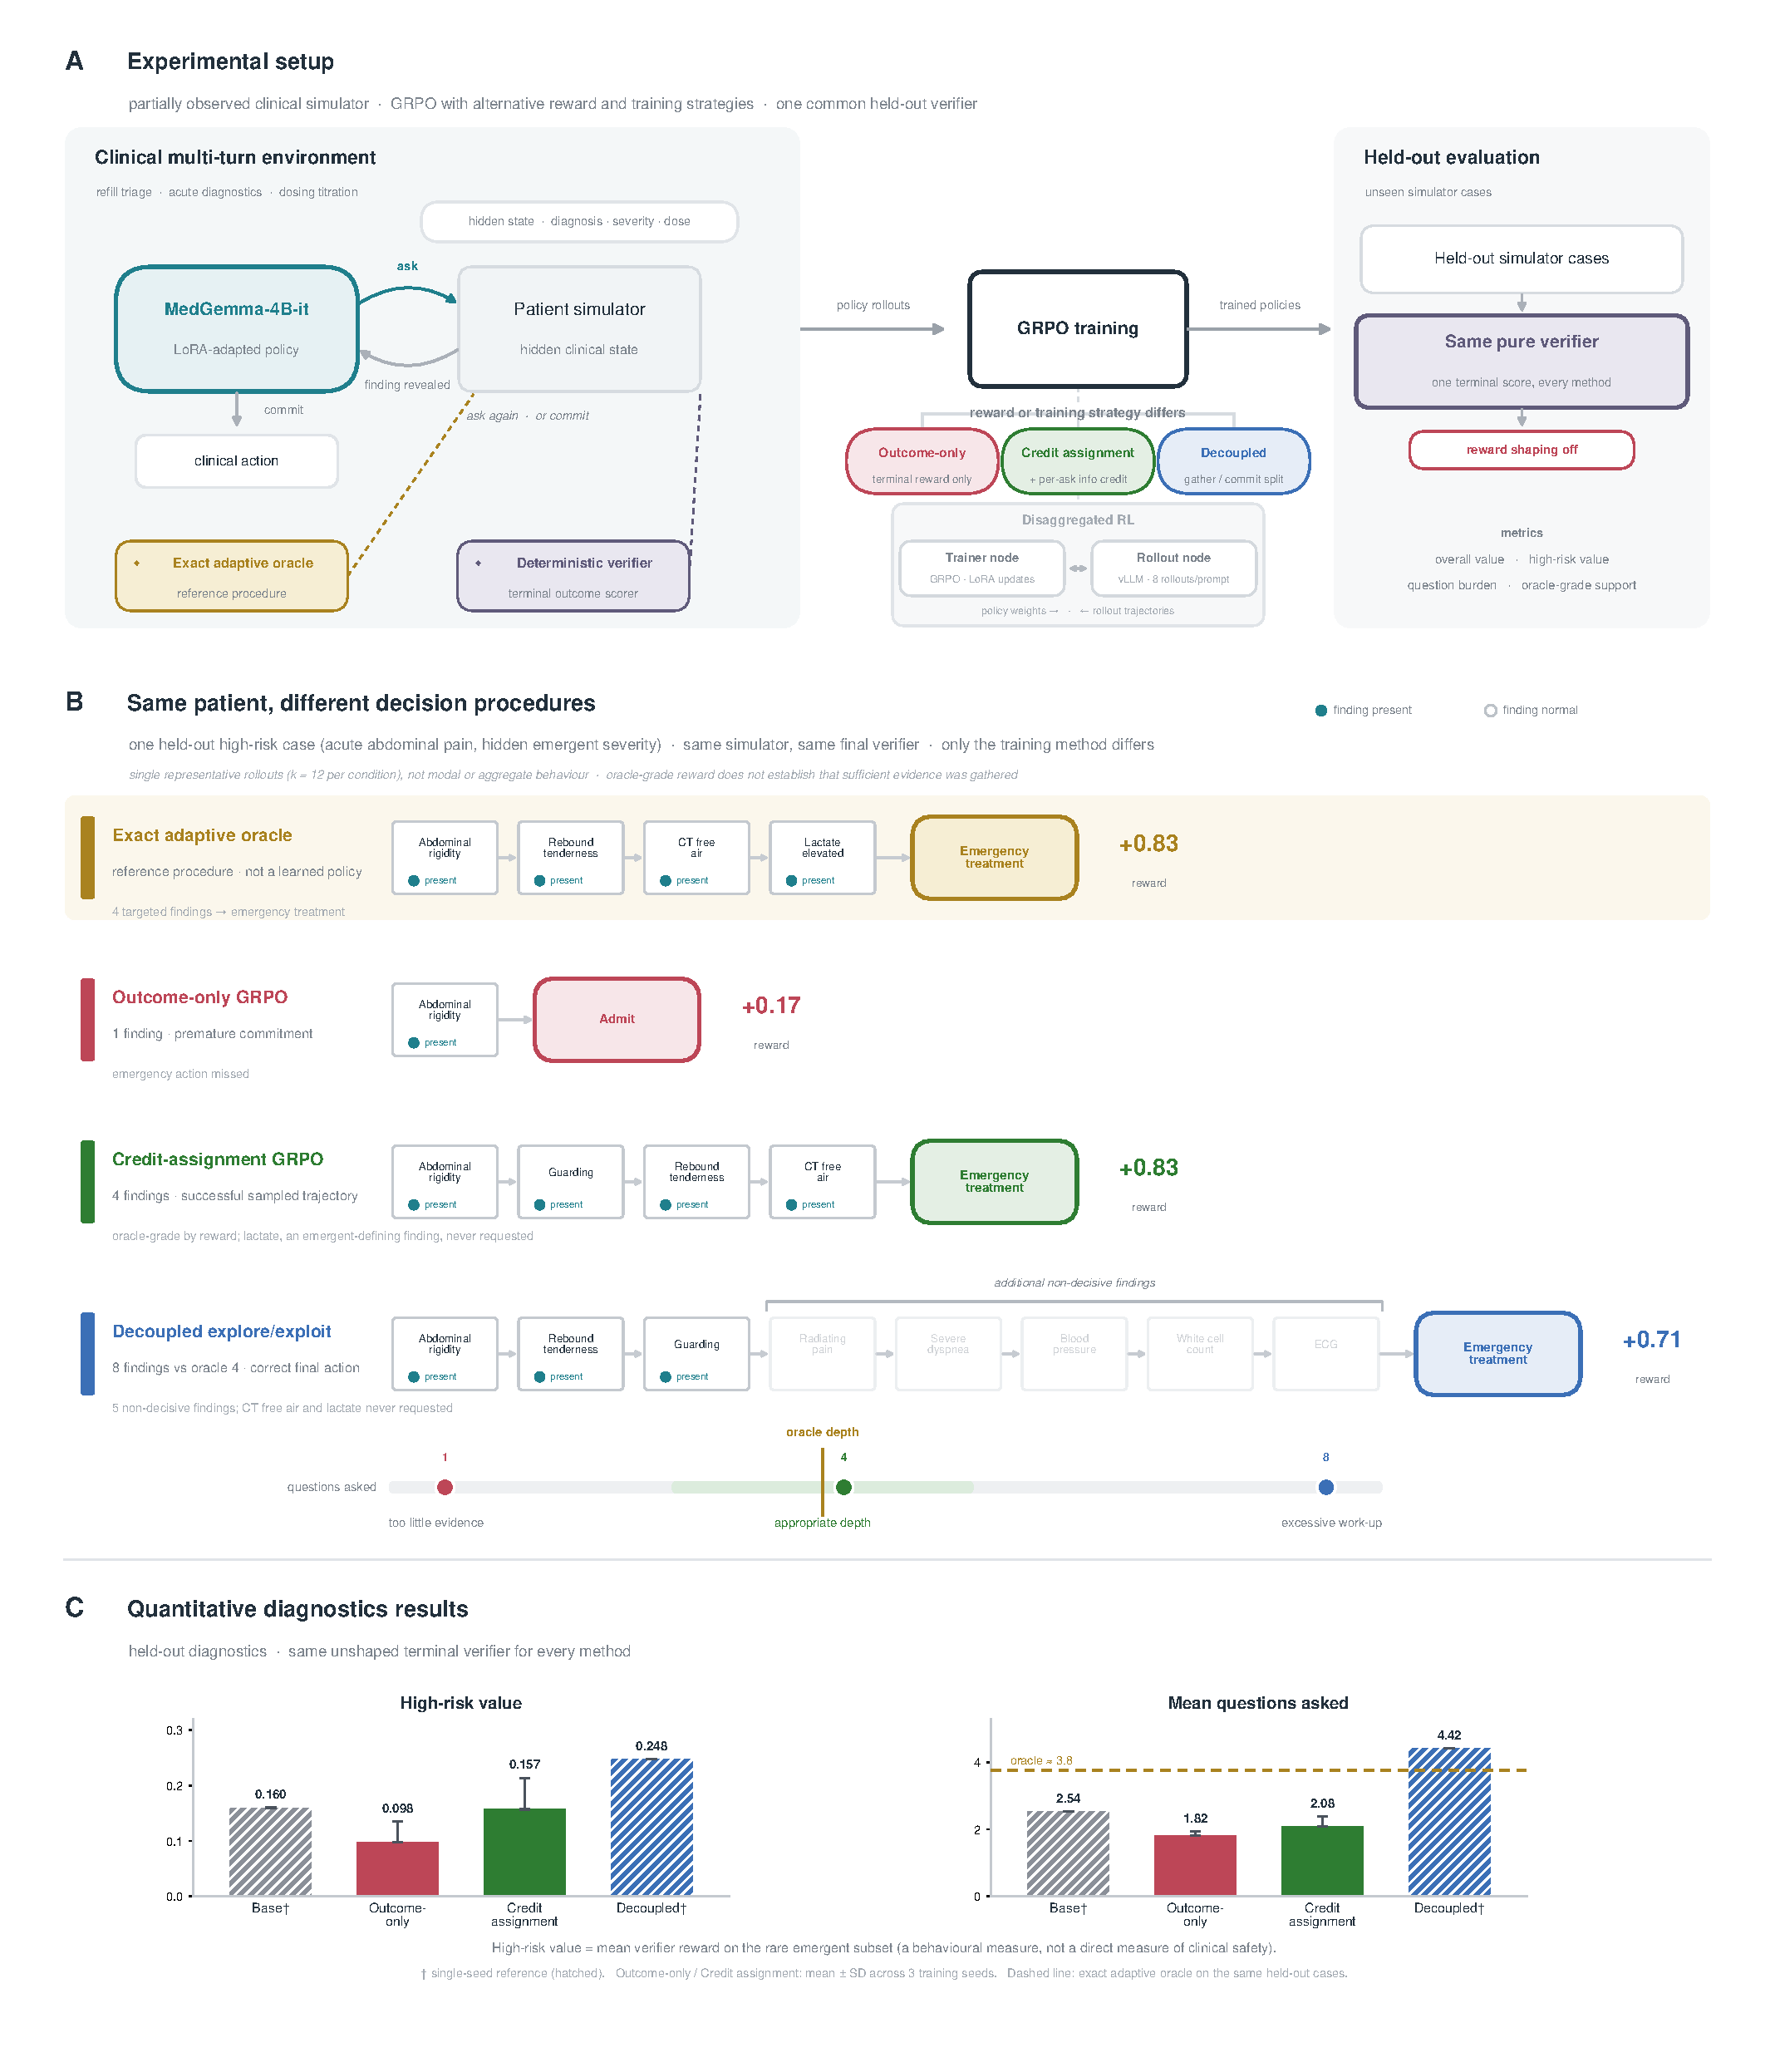
\includegraphics[width=\textwidth]{figs/figure1_combined.pdf}
  \caption{
  \textbf{Experimental framework and effects of reward design on clinical multi-turn decision procedures.}
  \textbf{A,} The MedGemma-4B-it policy, adapted with LoRA, interacts with a partially observed clinical
  patient simulator across medication-refill triage, acute diagnostics and dosing titration. The agent
  repeatedly asks for a clinical finding, receives the revealed result, and then either asks again or commits
  to a terminal clinical action; the underlying severity is never shown to the agent. Each controlled
  environment supplies two analytic reference structures rather than additional pipeline stages: an exact
  adaptive oracle (the reference information-gathering procedure) and a deterministic verifier (the terminal
  outcome scorer). GRPO training differs across methods only in the reward formulation -- outcome-only
  (terminal reward alone), credit assignment (terminal reward plus per-ask information-gain credit), and
  decoupled exploration/exploitation (gathering and committing optimised separately) -- with policy
  optimisation and rollout generation distributed across two compute nodes. All trained policies are then
  evaluated on held-out simulator cases under the same unshaped terminal verifier, with reward shaping
  disabled.
  \textbf{B,} Single representative rollouts from one held-out high-risk case (acute abdominal pain with a
  hidden emergent state) illustrate how information gathering and final action selection differ by training
  reward; rows are chosen to show distinct procedure classes and are not modal or aggregate behaviour for
  each method ($k=12$ rollouts per condition). The exact adaptive oracle requests four targeted findings
  before emergency treatment (reward $+0.83$). Outcome-only GRPO commits after a single finding and admits
  rather than treating, missing the emergency ($+0.17$). Credit-assignment GRPO reaches emergency treatment
  after four findings and is oracle-grade by reward ($+0.83$), although its evidence order differs from the
  oracle's. Decoupled exploration reaches the correct action only after eight requests, five of which are
  not decisive for the abdominal disposition, and the additional question cost reduces its reward
  ($+0.71$). Trajectory length is drawn to scale, so gathering depth is directly comparable across rows.
  \textbf{C,} Held-out diagnostics performance summarised by high-risk value -- the mean verifier reward on
  the rare emergent subset, a behavioural quantity rather than a direct measure of clinical safety -- and by
  the mean number of questions asked. Outcome-only and credit-assignment GRPO are reported as mean $\pm$
  standard deviation across three training seeds; the base model and decoupled GRPO are single-seed
  references (hatched bars, $\dagger$). The dashed gold line marks the exact adaptive oracle's mean question
  count on the same held-out cases ($\approx 3.8$). All values are computed with the same unshaped
  evaluation reward.
  }
  \label{fig:overview}
\end{figure*}
